\documentclass{article}

\usepackage{color}
\usepackage{textcomp}
\usepackage{setspace}
\usepackage[T1]{fontenc}
\usepackage{hyperref}
\usepackage{graphicx}
\usepackage{glossaries}
\usepackage{fullpage}

\graphicspath{{figures/}}

% \usepackage[lmargin=2cm,rmargin=2cm,tmargin=2cm,bmargin=2cm]{geometry}
%DRAFT - less paper
% \usepackage[lmargin=4cm,rmargin=2cm,tmargin=3cm,bmargin=2cm]{geometry}
%FINAL 1-sided
% \usepackage[lmargin=4cm,rmargin=2cm,tmargin=3cm,bmargin=2cm,twoside]{geometry}%FINAL 2-sided

%-----------------------------------------------------------------------
% red and blue boxes for drafting notes
%-----------------------------------------------------------------------
\definecolor{boxgray}{gray}{0.9}

\newcommand{\mycolorbox}[3]{
 \vspace{5mm}
 \noindent
 \fcolorbox{#1}{#2}{
   \begin{minipage}[l]{0.95\textwidth}
     \color{#1}
     #3
   \end{minipage}
 }
 \vspace{3mm}
}

\newcommand{\myredbox}[1]{\mycolorbox{red}{boxgray}{#1}}
\newcommand{\mybluebox}[1]{\mycolorbox{blue}{boxgray}{#1}}
\newcommand{\mygreybox}[1]{\mycolorbox{black}{boxgray}{#1}}
\newcommand{\mywhitebox}[1]{\mycolorbox{black}{white}{#1}}

\newcommand{\crumbs}[1]{\myredbox{#1}}
\newcommand{\excrumbs}[1]{\mybluebox{#1}}
\newcommand{\draft}[1]{\mygreybox{#1}}

%------------------------------------------------------------------------------
% setting for displaying python code in its own environment
%------------------------------------------------------------------------------
\usepackage{listings} %for code listings
\usepackage[scaled]{beramono} %nicer monospace font for code listing

\renewcommand{\lstlistlistingname}{Code Listings}
%\renewcommand{\lstlistingname}{Code Listing}% default is 'Listing'

\definecolor{lstgray}{gray}{0.2}
\definecolor{lstgreen}{rgb}{0,0.5,0}
\definecolor{lstmaroon}{rgb}{0.4,0.4,0.4} % comments
\definecolor{lstpurple}{rgb}{0.5,0,1.0}
\definecolor{lstdarkpurple}{rgb}{0.2,0,0.5}
\definecolor{lstdarkblue}{rgb}{0,0,0.6}

\lstnewenvironment{python}[1][]{
\lstset{
language=python,
basicstyle=\ttfamily\footnotesize\setstretch{1},
stringstyle=\color{lstdarkpurple},
showstringspaces=false,
alsoletter={1234567890},
otherkeywords={\ , \}, \{},
keywordstyle=\color{black},
emph={access,and,break,class,continue,def,del,elif,else,%
except,exec,finally,for,from,global,if,import,in,is,%
lambda,not,or,pass,print,raise,return,try,while},
emphstyle=\color{blue}\bfseries,
emph={[2]True, False, None, self},
emphstyle=[2]\color{lstgreen},
emph={[3]from, import, as},
emphstyle=[3]\color{blue},
upquote=true,
morecomment=[s]{"""}{"""},
commentstyle=\color{lstmaroon}\slshape,
%emph={[4]1, 2, 3, 4, 5, 6, 7, 8, 9, 0},
%emphstyle=[4]\color{red},
literate=*{:}{{\textcolor{lstdarkblue}:}}{1}%
{=}{{\textcolor{lstdarkblue}=}}{1}%
{-}{{\textcolor{lstdarkblue}-}}{1}%
{+}{{\textcolor{lstdarkblue}+}}{1}%
{*}{{\textcolor{lstdarkblue}*}}{1}%
{!}{{\textcolor{lstdarkblue}!}}{1}%
{(}{{\textcolor{lstdarkblue}(}}{1}%
{)}{{\textcolor{lstdarkblue})}}{1}%
{[}{{\textcolor{lstdarkblue}[}}{1}%
{]}{{\textcolor{lstdarkblue}]}}{1}%
{<}{{\textcolor{lstdarkblue}<}}{1}%
{>}{{\textcolor{lstdarkblue}>}}{1},%
framexleftmargin=1mm, framextopmargin=1mm, 
frame=Tb,%rulesepcolor=\color{blue},
#1 }}{}
%------------------------------------------------------------------------------

\title{A Testbed Application for Scaling Location-Based Social Networking Applications}
\author{Allan Jones}
\begin{document}
	\maketitle

%------------------------------------------------------------------------------
%%%%% Abstract
%------------------------------------------------------------------------------
\begin{abstract}
	Modern social networking services with a large user-base are capable of generating immense amounts of data. This presents challenges to the developers of these services, who are responsible for ensuring they are capable of scaling to an increase in users and traffic. This report presents the design and implementation of a solution built upon Google App Engine for organising data for a mobile, location-based social networking application; the goal of which is to limit repetitive and costly server-side processing. Early results of testing indicate that it is effective in reducing the amount of server-side processing overhead, but that further investigation of the Google App Engine framework is required in order to optimise the solution for such problem domains.
\end{abstract}

%------------------------------------------------------------------------------
%%%%% Introduction
%------------------------------------------------------------------------------
\section{Introduction} % (fold)
\label{sec:introduction}

% \crumbs{Cite something that covers online marketplaces vs. "distributed applications"? What is the proper term for this?}

The popularity of web-enabled mobile devices has seen a significant increase in the last couple of years. This rise in popularity can be largely attributed to the the success of online marketplaces, such as the Apple App Store\footnote{Apple App Store: \url{http://www.apple.com/iphone/apps-for-iphone/}} and Android Market.\footnote{Android Market: \url{http://www.android.com/market/}} These online marketplaces provide mobile device owners a means of discovering and acquiring applications that is centralised, allowing applications to be consumed with greater ease than the traditional distributed model.

Amongst the most downloaded and used applications available through these online marketplaces are those which utilise already well established social networking services, such as Facebook and Twitter. This has led to a substantial increase in the amount of traffic for these services, as users are no longer required to be at a computer in order to use them.

Traditionally, the developers of social networking services built as web applications have faced substantial challenges relating the capacity of the application to scale to handle a user-base that has hit critical mass. These challenges include things such as being able to handle large numbers of concurrent user requests, ensuring near-optimal server-side processing across an extensive data set and fast delivery of content to the end-user, just to name a few.

Studies of the usage patterns of mobile applications indicate that, on average, users spend a small amounts of time using an application. This phenomenon presents greater challenges for the developers of social network services, who must ensure that the service is responsive enough to engage their mobile user-base in a limited time window.

Platforms for providing web-scale computing such as Google App Engine\footnote{Google App Engine: \url{http://code.google.com/appengine/}} and the Amazon Elastic Compute Cloud (EC2)\footnote{Amazon Elastic Compute Cloud (EC2): \url{http://aws.amazon.com/ec2/}} offer an infrastructure for building applications that utilise massive amounts of processing power. These services allow developers to easily scale applications to meet increases in traffic, by allowing control over the amount of processing required by their applications. While these platforms provide an attractive offering for developers looking to build large-scale applications, it is unknown whether they are a viable back-end for all kinds of applications, or to a distinct subset.

This report introduces a prototype mobile location-based social networking application. Following this is the design and implementation of a strategy for organising large quantities of data generated by the application that is built using the Google App Engine platform. Finally, we discuss the initial results of testing the organisation strategy developed and possibilities for further research related to improving the strategy.

% section introduction (end)

%------------------------------------------------------------------------------
%%%%% Technical Detail
%------------------------------------------------------------------------------
\section{Technical Detail} % (fold)
\label{sec:technical_detail}

\subsection{Prototype Mobile Application} % (fold)
\label{sub:prototype_mobile_application}

As a starting point for developing the data organisation strategy, a prototype mobile application was created. The application was built using the Apple iOS SDK,\footnote{iOS SDK: \url{http://developer.apple.com/devcenter/ios/}} which operates on the iPhone and iPad devices developed by Apple. The purpose of the application was to model the usage of a social networking service and to act as a producer and consumer of data stored on a server. The following sections provide an overview of the prototype application, including its primary function and the data model upon which it is built.

\subsubsection{How the Application Works} % (fold)
\label{ssub:how_the_application_works}

The prototype was developed as a location-based social networking application for mobile devices. The primary function of the application is to allow a user to create a message at a particular location within the world, which is received by other users that are present at the same location at any given time after the message has been created. This is achieved through the use of the phone's built-in GPS, which allows the phone to determine the latitude/longitude coordinate for its current location. Each time the phone detects a significant change in location, this value is automatically updated. Once a location change has been detected, the application will register its new location with a request to a central server, which will in turn send the messages for that location as a response to the phone.

A hypothetical example application's usage would be one in which a message is left by a user in Times Square, NY and later received by a user who enter the region; as illustrated in Figure~\ref{fig:location_based_messaging}. In this example, \emph{User 1} leaves a message at 11:00 AM on a given day, indicating that there is a sale on coffee at a nearby caf\'e. The message is sent to the server, which stores the message content and the location from which it was sent. A 1:30PM on the same day, \emph{User 2} enters the area within which the message was left. This triggers a request to the server to indicate the user is now at this location. As a response to the location update, the server retrieves the message that was left at the location by \emph{User 1} and the message is sent as a response to \emph{User 2}.

\begin{figure}
\begin{center}
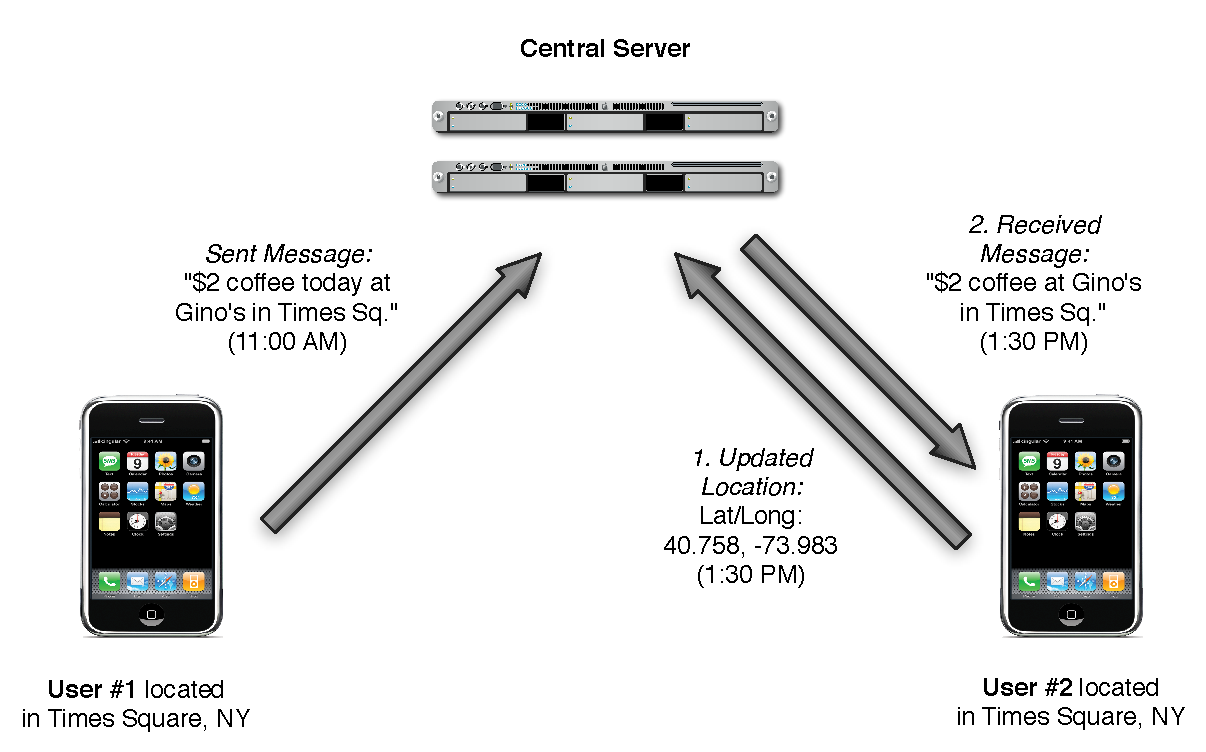
\includegraphics[width=12cm]{location-based-messaging.pdf}
\caption{User \#1 leaves a message in Times Square, NY at 11:00 AM. At a later time (1:30 PM), User \#2 enters the region and receives the message that was left. This information is relayed by the server, which maintains a collection of the messages associated with a given location.}
\label{fig:location_based_messaging}
\end{center}
\end{figure}

% subsubsection how_the_application_works (end)

\subsubsection{Data Model} % (fold)
\label{ssub:data_model}

The prototype's domain model consists of three core entities: \emph{User}, \emph{Message} and \emph{Location}, as represented in Figure~\ref{fig:domain_model}. The \emph{User} entity represents a mobile device owner that has installed and registered with the application. Each \emph{User} has a unique \emph{Username} that identifies them within the application. The \emph{Message} entity represents a message created by an \emph{Author} (i.e. a \emph{User} that created it). Each message has an associated \emph{Title} and \emph{Content} (i.e. message), as well as a time at which it was created \emph{Date Created} and the \emph{Location} at which it was created. Finally, the \emph{Location} entity consists of a \emph{Latitude} and \emph{Longitude}, which represent it's latitude/longitude coordinate.

\begin{figure}
\begin{center}
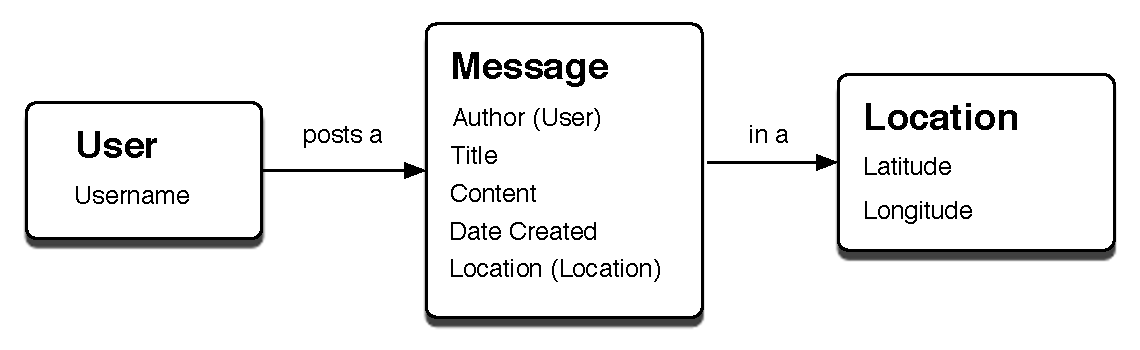
\includegraphics[width=12cm]{domain-model.pdf}
\caption{The domain model for the prototype application. \emph{Users} are responsible for the creation of \emph{Messages}, which are associated with a particular \emph{Location} (latitude/longitude coordinate).}
\label{fig:domain_model}
\end{center}
\end{figure}

% subsubsection data_model (end)

% subsection problem_details (end)

\subsection{Solution Details} % (fold)
\label{sub:solution_details}

\subsubsection{Constraints} % (fold)
\label{ssub:constraints}

Prior to the development of a potential server-side component for content delivery, appropriate constraints were defined to assess the effectiveness of a given solution. The constraints were defined with the intention of limiting both the volume of information transmitted between the device and the server and the time taken for data transmission. The constraints are as follows:

\begin{description}
	\item[Messages per request] Users are able to receive a maximum of 50 messages for a given request
	\item[Message size] The body content of a message must be no longer than 250 characters
	\item[Response size] A single request to the server should yield no more than 500 KB worth of response data
	\item[Total processing time] The time taken to initiate a request from the device to server, receive a response and render content should take no longer than 5 seconds
	\item[Response guarantee] Provided there is data available for a location, a request should never yield no response data
\end{description}

% subsubsection constraints (end)

% subsection solution_details (end)

\subsubsection{Message Grouping} % (fold)
\label{ssub:message_grouping}

Delivering individual messages from the server to the device for a given request would incur unnecessary processing overhead if there was a number of messages associated with a location. Also, if a user was required to be at an exact latitude/longitude coordinate in order to receive a message, the message may never be received as the value of the coordinate is continuous, rather than discrete. Therefore, the approach of grouping adjacent messages together was taken, allowing the delivery of a payload of messages.

In the case of the prototype, there are two factors of adjacency for messages, \emph{location} and \emph{time}. As location is the primary factor for adjacency, messages were grouped together according to a common geospatial region. Additionally, the messages were organised according to a chronological timeline.

% paragraph message_grouping (end)

\subsubsection{GeoModel} % (fold)

To determine the geospatial regions by which messages were grouped, the GeoModel API was utilised, the purpose of which is to allow indexing and querying of geospatial data within Google App Engine.\footnote{GeoModel API: \url{http://code.google.com/p/geomodel/}} The API provides a geospatial representation of the earth that is similar to that of geohashing.\footnote{Geohashing: \url{http://en.wikipedia.org/wiki/Geohash/}}

The API represents the world as a rectangular 4x4 grid, with each cell within the grid being marked by a character from 0-f. Within each of those cells is another 4x4 grid of cells. This grid definition within a cell is recursive, with each grid cell possessing 4$x$4 cells to a resolution of 16. An example of the recursive definition of cells in highlighted in Figure~\ref{fig:geocell_resolutions}. The full range of coordinates from -90,-180 to 90,180 fall within cells 0-f, at a cell resolution of 1. Cell 7 has a direct child grid encompasses cells 70-7f, containing coordinates -45,90 to 0,180.

\begin{figure}
\begin{center}
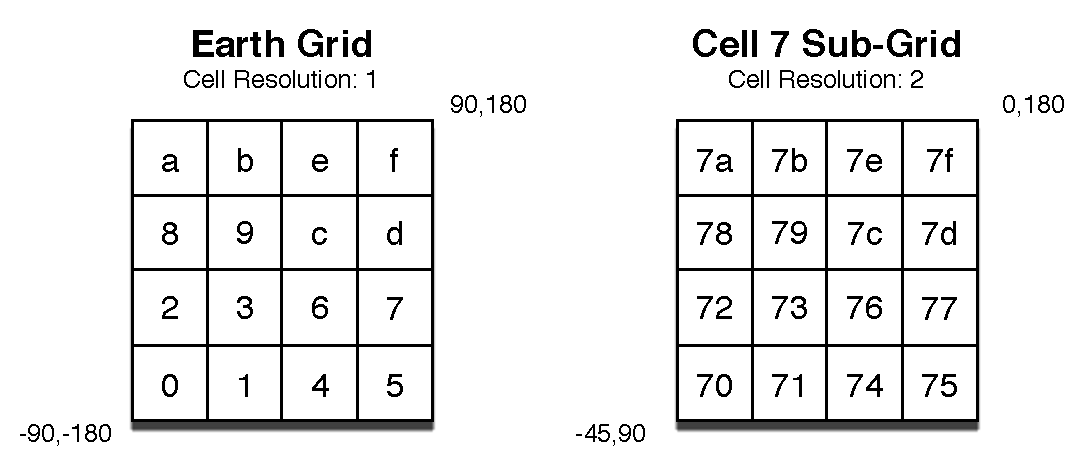
\includegraphics[width=12cm]{geocell-resolutions.pdf}
\caption{A breakdown of geocell division according to latitude/longitude coordinates. Shown on the left is the 4x4 grid for the lowest possible geocell resolution, which covers the full range of latitude/longitude coordinates. On the right, the immediate child grid of cell 7 is shown, with a resolution of 2, covering a latitude/longitude range of -45,90 to 0,180.}
\label{fig:geocell_resolutions}
\end{center}
\end{figure}

% \excrumbs{Using this approach, we can define an area of space this is elastic, i.e. we can define a bigger or smaller space simply by combining grid cells.
% \textbf{TODO: Need the measurements for upper and lower resolution limit}}

To define a resolution suitable for data retrieval for mobile devices, an experiment was conducted to measure the GPS accuracy of a number of iPhones. The investigation found that, on average, the locations determined by the phone's GPS were accurate to within 500 metres. To cater for this lack of precision a cell resolution of 8 was used.

\subsubsection{Message Buckets} % (fold)

For storing grouped messages together the approach taken was to create a large number of buckets that would hold the message content. The buckets represent small, fixed-capacity containers that are filled with message content. Once filled to capacity, a new bucket is created to hold any messages that didn't fit into the bucket. While the number of messages stored in a single bucket could be any number, big or small, it is intentionally kept small. This is done to ensure that transmission costs for a single bucket are low. It also allows a number of buckets to be collated to be sent as a response to the user. By sending multiple, small buckets, there is a guarantee that of \emph{n} total buckets that are part of a response, \emph{n-1} buckets will have a full payload. If a single, large bucket were sent as a response to the phone, there would be no guarantee how many messages it would contain. 

When filling the buckets with messages, the message content is stored within the buckets in a data interchange format, as opposed to the runtime objects that represent the messages. The reason for this is so that the data is provided to the phone is a format that it can easily understanding and consume. In this case, the JSON\footnote{JSON: A data interchange format in which data is specified using the JavaScript object notation \url{http://www.json.org/}} data interchange format was used, due to the availability of APIs for handling JSON across multiple and platforms programming languages. The messages are serialized prior to being put in the bucket to reduce the need to serialize message content any time the contents of a bucket are sent as a response to the device.

\begin{figure}
\begin{center}
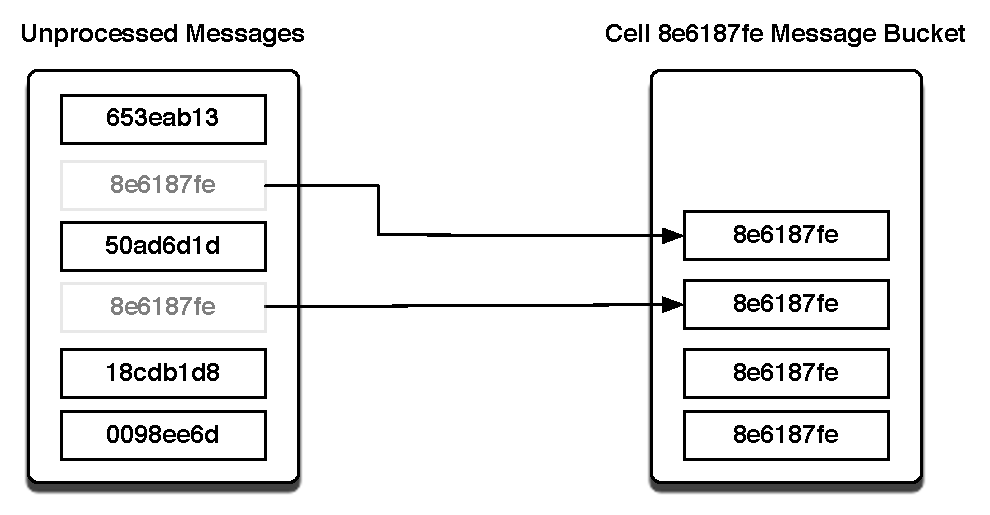
\includegraphics[width=12cm]{geocell-bucket-filling.pdf}
\caption{Messages at a location within the 8e6187fe cell are taken off the unprocessed message queue and placed in the message bucket for the cell. Labels on the messages denote the geocell that their associated location is within.}
\label{fig:geocell_bucket_filling}
\end{center}
\end{figure}

\subsubsection{Preparation of Buckets} % (fold)
\label{ssub:preparation_of_buckets}

The preparation of buckets to accommodate new messages should occur at regular timed intervals or be triggered by some other event. In this case, a scheduled cron job that ran the bucket preparation algorithm 10 times per minute was used. The Python code for the algorithm used to allocate messages to buckets is shown in Figure~\ref{fig:bucket_preparation_algorithm}. The algorithm is composed of the following steps:

\begin{figure}
\begin{center}
\begin{minipage}{5.5in}%
\label{fig:message_processing_pseudocode}
\begin{algorithmic}
\STATE messages = get messages to process

\STATE top = get top bucket

\STATE fill bucket with messages(current top, messages)

\WHILE{messages > 0}
	\STATE new top = create new bucket
	\STATE fill top bucket with messages(messages)
	\STATE link buckets(top, new top)
	\STATE top = new top
\ENDWHILE
\end{algorithmic}
\end{minipage}
\end{center}
\end{figure}

\begin{description}
	\item[Retrieve unprocessed message hash] {Messages are retrieved from the data store to be processed and allocated to buckets. The call to \texttt{get\_unprocessed\_message\_hash()} encompasses the following two actions:

	\begin{enumerate}
		\item A pre-defined number of unprocessed messages are retrieved from the data store. The number chosen was 100 messages per request. The retrieved messages are be ordered by the time at which they were created.
		\item The messages fetched from the data store are stored in a dictionary mapping the message (values) to the geocells in which they are present. This step is included to pre-allocate messages to a bucket, to avoid multiple trips to the data store in cases there are a number of messages to go in buckets.
	\end{enumerate}}
	
	\item[Allocate messages to buckets] Each of the messages is allocated to a bucket for the geocell within which it was created. The following steps are performed for each entry in the geocell to message list dictionary:
	
	\begin{enumerate}
		\item Get the current top bucket for the geocell. If no buckets exist for the geocell then a bucket is created and assigned the status of top bucket.
		\item Fill the bucket with the messages intended for the geocell using the first message index as an offset for the messages to be allocated to the bucket. If the number of messages exceeds the maximum number of messages that the bucket is able to hold, then the bucket is filled only to its full capacity.
		\item Persist changes to the bucket to the data store
		
		\item
		{
			While there are messages left to be allocated:
			
			\begin{enumerate}
				\item Clear the top bucket's status (indicating it is no longer the top)
				\item Create a new bucket
				\item Flag the new bucket as being the top bucket
				\item Fill the new bucket to capacity with messages
				\item Link the buckets to one another by ID 
				\item Persist changes to both the old and new bucket
				\item Assign the new bucket to the top bucket variable
			\end{enumerate}
		}
	\end{enumerate}

\end{description}

\begin{figure}
\begin{center}
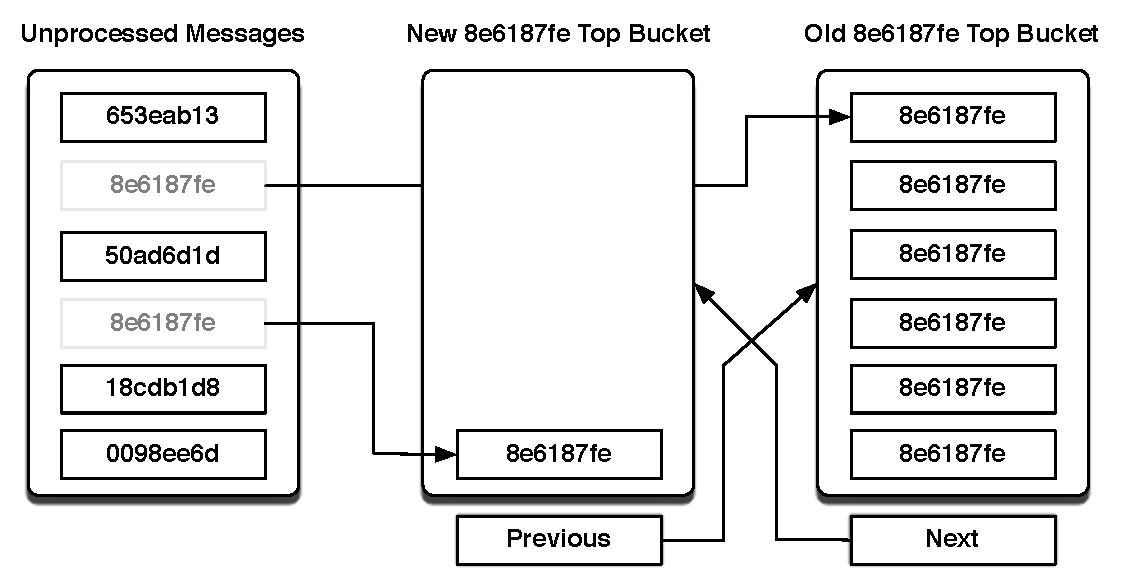
\includegraphics[width=12cm]{geocell-new-bucket.pdf}
\caption{Once the top bucket for a geocell has been filled to capacity, a new bucket is created. At this point, the newly created bucket is assigned the top bucket status and is associated with the old bucket (Previous), while the old bucket is associated with it (Next).}
\label{fig:geocell_new_bucket}
\end{center}
\end{figure}

%------------------------------------------------------------------------------
\begin{figure}
\begin{center}
\begin{minipage}{5.5in}%
\begin{python}
	% caption={Bucket preparation algorithm in Python},label={code:ec_GA} 
def prepare_buckets_for_messages():
  # Get a hash of geocell -> unprocessed messages
  geo_msg_hash = get_unprocessed_message_hash()

  # For each geo-cell to message hash entry
  for cell, msg_hash in geo_msg_hash.items():
    # Store the number of messages to process
    unprocessed_messages = msg_hash["count"]
    total_messages = unprocessed_messages
    # Get the top bucket
    top = get_top_bucket(cell, msg_hash["geocells"])
    # Fill the bucket, getting the number of messages
    # put in the bucket. Use the first message index (0) as
    # as the index from which to fill the bucket from
    count = fill_bucket(top_bucket, msg_hash["messages"], 0)
    # Decrease the messages left to process
    unprocessed_messages -= message_count_for_bucket
    # Persist changes to the top bucket
    top.put()

    # While there are still messages to store, create a bucket,
    # mark it as top and store as many messages as possible in it   
    while unprocessed_messages > 0:
      # Mark the current top bucket as not being
      # the top bucket any longer
      top.status = 0
      # Make a new bucket
      new_bucket = new_public_bucket(geocell)
      # Flag the new bucket as the top
      new_bucket.status = PUBLIC_BUCKET_STATUS_TOP
      # Get the index of the next message to be processed
      next_index = total_messages - unprocessed_messages
      # Fill the bucket and store the no. of messages added
      count = fill(new_bucket, msg_hash["messages"], next_index)
      # Decrease the messages to process according to
      # number stored in bucket
      unprocessed_messages -= count
      # Associate the buckets with one another by ID
      top.next_bucket_id() = new_bucket.id()
      new_bucket.prev_bucket_id() = top.id()
      # Persist changes to top and new buckets
      top.put()
      new_bucket.put()
      # Set top bucket as the new bucket created
      top = new_bucket
\end{python}
\end{minipage}
\caption{Code snippet showing the algorithm used to prepare buckets for messages within geocells. Messages are first hashed to their associated geocell, then buckets are filled and created (as necessary) until all messages have been processed.\label{fig:bucket_preparation_algorithm}}
\end{center}
\end{figure}
%------------------------------------------------------------------------------

% subsubsection preparation_of_buckets (end)

% section technical_detail (end)

%------------------------------------------------------------------------------
%%%%% Discussion
%------------------------------------------------------------------------------
\section{Discussion} % (fold)
\label{sec:discussion}

\subsection{Preliminary Results} % (fold)
\label{sub:preliminary_results}

Preliminary results from the testing of the proposed solution have been encouraging. The allocation of messages to buckets has resulted in a dramatic increase in the performance of retrieving and delivering messages. These benefits would become even more apparent as the user-base scales. However, the performance of the bucket preparation mechanism is currently a bottleneck that is prohibiting the application from being applied to the large-scale for which it was intended.

Testing of the strategy on a local deployment yields satisfactory processing times, leading to the belief that when deploying to Google App Engine it should perform equally well. However, when deployed to App Engine, the allocated processing resources and cumulative processing time (a measure of total CPU usage calculated by App Engine) increases dramatically. Further investigation of the problem reveals that writes to App Engine's distributed data store are of very high latency and a large performance penalty is incurred when multiple writes occur.

% subsection preliminary_results (end)

\subsection{Future Work} % (fold)
\label{sub:future_work}

Based on the preliminary results of testing the strategy, the logical next step is to address the performance concerns of interacting with Google App Engine's data store. Primarily, the focus will be on ways of managing writes to the data store in order to limit the costs associated with an excessive number of writes. This will include investigating ways in which writes can be minimised, as well as batch-writing to allow larger amounts of persistence to occur in a single transaction.

Following this will be efforts to make improvements to the speed of the delivery of data from the server to the device. This could focus on the practicalities of using App Engine's implementation of caching to build an effective caching layer for applications in the domain of social networking. In particular, this would focus on how much data should be cached and the format in which it should be cached to enable the fastest possible throughput while incurring low processing overheads. This would also require exploration of approaches to keeping the caching layer in synch with the data store.

Another possible topic of research is that of the choice of data interchange format for the data exchanged between the device and server. Lightweight alternatives to the JSON interchange format currently used, such as Protocol Buffers, BSON or Apache Thrift may offer substantial benefits by reducing processing overhead for serialization/deserialization and the amount of bandwidth consumed through the transmission of data.

% subsection future_work (end)

% section discussion (end)

%------------------------------------------------------------------------------
%%%%% Conclusion
%------------------------------------------------------------------------------
\section{Conclusion} % (fold)
\label{sec:conclusion}

In this report, a prototype mobile location-based social network application was introduced. Using the application as a base, the design and implementation of a strategy for organising user data built using the Google App Engine framework was presented; the goal of which is to reduce repetitive and costly server-side processing. Following this, some preliminary results of testing the implementation of the strategy deployed to Google App Engine were discussed. The results indicated that the strategy was successful in its objective of reducing repetitive and costly processing. However, the write latency associated with  the Google App Engine data store arose as a concern, making it an obvious threat to the ability of the application to scale. The next step is to address the efficiency of write performance by investigating the possibility of batch processing the writes to reduce the numbers of hits to the data store. Additionally, ways of improving the performance of the delivery of content such as caching and alternative lightweight data interchange formats will be explored.

% section conclusion (end)

\end{document}

% \crumbs{Need some numbers indicating the performance levels here}
% 
% \crumbs{Need to expand this section to include more detail of the results of the solution. May want to include a small Results section which highlights the results and provides more ground for discussion.}

% \crumbs{The following paragraphs need to be a little clearer in describe the problems faced and what the solution aimed to address. \textbf{Lowering costly and avoidable server-side processing and providing fast retrieval times for geo-located data.}}

% \excrumbs{
% In this report, the issues of scalability in social networks was introduced. A prototype for a mobile, location-based social networking application was described to set the context.}

% \excrumbs{
% Using this application as a base, the design and implementation of a server-side component built using Google App Engine was presented, with the aim of addressing some of these issues.
% }

% \draft{In choosing how to effectively group the messages, it was important to understand the criteria according to which messages are retrieved. For this problem, the messages are retrieved according to both the location of a retriever, as well as point in time for which they are interested in. In most cases, this will be the current time, however it was necessary to also consider the possibly of the retrieval of messages that were created at some point in time that is outside a definition of time that can be considered time.}
% 
% \draft{If we were to group according to continuous points (i.e., latitude/longitude), there are potentially infinite locations that could be represented. While this can be resolved by using lat/long values that are trimmed to a given precision, it is more sensible and closer to the problem to represent the earth's landscape as a collection of geospatial areas, which contains the latitude/longitude coordinates that the messages are relevant for.}

 % as a driver for addressing the problem of organising data with the goal of lowering server-side processing overhead. Motivated by this application, the design an implementation for data organisation was presented as a starting point for investigation into the problem. Using the 

% The increase in social networking traffic brought about by mobile usage has magnified the difficulty of the challenges associated with scalability, with mobile consumption accounting for a large 

% % he traffic for these services has now increased substantially, with mobile traffic now accounting for a large proportion of all user activity.
% 
% \excrumbs
% {
% Traditionally, social networking services have faced problems associated scalability as the volume of users and traffic increases.
% 
% \begin{itemize}
% 	\item Handling large numbers of concurrent user requests
% 	\item Server-side processing overhead due to amount of data
% 	\item Ensuring a fast response time for user requests
% \end{itemize}
% }

% These challenges have become even more prevalent with the increased accessibility of these services through the use of mobile devices.
% 


% \crumbs{Figure here that shows a comparison between downloading from different sources compared to online marketplaces...try to demonstrate ease of discovery/acquisition in the new model}



% Applications such as those based on social networks have reversed the traditional model of content production by instead giving that capability to users, allowing for a more diverse and engaging online experience. This is particularly evident with the increase in mobile devices, which allow users to produce content based on their experiences as they happen.

% While this is obviously advantageous from a user experience point-of-view, it increases the difficulty that was already faced in providing high-availability and fast access to data for consumers.

% \crumbs{Following paragraph should be bit clearer...be concise...challenges are that not everyone wants the same data with the same frequency, so we have to be more careful }

% Social networking applications often have non-trivial conditions and rules which govern what a particular user should be able to see at a given point in time. This includes things such as the other users a given user is associated with, personal preferences tailored to the users individual tastes and privacy settings which determine whether the user is authorised to access the content. Because of this, traditional approaches towards improving availability for users and decreasing the time taken to retrieve data, such as data organisation and caching, requires more careful consideration.
% 
% \crumbs{Should move this up a bit...it is the high-level problem we're facing}

% \excrumbs{Research into the usage patterns of users of applications on devices show that users spend a small amount of time using the apps each time they are used. This means that developers of the applications have a limited amount to engage their users. }

% In order to cope with the inevitable issues with scaling that come with increased popularity in such applications, developers must endeavour to build more sophisticated mechanisms, so as to ensure a fast and responsive experience to end-users of the application.

% In this report, a location-based social networking application is introduced as a catalyst for investigating the problem of organising large quantities of related data to limit repetitive server-side processing.
% 
% Using this problem as a guide, the design and implementation of a solution built upon Google App Engine that organises frequently accessed data using a geospatial grid is described; the motivation of which is to provide a starting point for exploration in the area of scalability for mobile web traffic, particularly that relating to large-scale social networks.
% 
% Following the description of this solution is a some initial results of testing the implementation are presented. Using the results, a discussion of how the solution may be improved and other possible related research topics

% In this report, a prototype back-end built on Google App Engine for handling data for a mobile location-based social networking application is presented. 

% We present a prototype mobile application and server-side "component" built on Google App Engine

% Unlike traditional online content, this data may only be relevant to a particular user according to a specific set of conditions.

% Dealing with such large amounts of data with often complex rules governing how it is delivered to a user requires the adoption of more thoughtful strategies to minimise associated processing overhead and costs.

% This report presents the design and implementation of a solution for organising data for a mobile, location-based social networking application; the goal of which is to limit repetitive and costly server-side processing.
% 	
% 	Accompanying the solution described is a discussion of the implications of the design and implementation choices made, along with a discussion of possibilities for further research endeavours in this problem space.

% - Social media applications are become integrated within our daily lives
% 
% - Effective means of communication and information discovery
% 
% - Most of them are free...users like free stuff!
% 
% - Mobile applications enable users to be out and about while surfing the web, something that wasn't really possible previously
% 
% - There is stuff to do when users are out and about, which social media apps can enhance

% - Some social media apps are super rich in content and have a substantial base of users
% 
% - This is a great thing, but somewhere this data needs to be stored (huge amounts of data!)
% 
% - Additionally, not every user is going to want every bit of data
% 
% - A search for personalised data (i.e. data that an individual user cares about) at a large-scale can be computationally expensive and slow (users don't like to wait!)
% 
% - Caching alleviates this problem to some extent (allows computations to occur a smaller number of times, with the results stored -- caching tier is much lower latency than the datastore)
% 
% - Problem is, that this doesn't come cheap
% 
% - Cached data is not persistent (caching tier is separate from DB)
% 
% - Need to ensure cache is not invalid (we need to provide users with the data they want)
% 
% - As the number of users increases, it becomes less practical to provide high-availability/throughput personalized information
% 
% - We need to make trade-offs, based on the problem space (no of users, user usage patterns, distribution of data -- location-based)
% 
% 
% \textbf{Focus should be on mobile devices}

% - Mobile devices are becoming more and more sophisticated, especially with advances in GPS technology, which enables the device to know where it is at a given time. This capability holds the potential of allowing application developers to enrich their applications by enabling their application to perform functionality that is location sensitive. Some practical examples of this include the ability for storefronts to trigger a notification on a end-user's device when they are in a location that is nearby, telling them that there is a sale on \textbf{TODO: Put another practical example in here}.
% 
% \textbf{Paragraph regarding the need for apps to be responsive, due to the tendency of users to not spend all that long actually using the app...highlight that it is even more important for web-enabled applications, which rely on the internet for their content}
% 
% \textbf{need to cite a source here...a study of how long user's typically use apps for}
% 
% \textbf{Modern online social networks are particularly content rich...while a small number of users of the social networks will only account for a relatively small amount of content, as the networks to greater numbers of users, so does the content, making the retrieval of content of more difficult and more resource intensive}
% 
% \textbf{This report presents a possible solution to the problem of organising data for location-sensitive social networking application}


% Objectives of the report:
% - Outline (in some detail) the problem faced by high-traffic internet services when providing data to a lot of different people
% 
% - Be more specific to the problem we face (mobile social networking application, location-based data retrieval)
% 
% - Cover some of the general guidelines to solving these kinds of problems
% 
% - Describe scenarios which we are likely to encounter
% 
% - Describe and implement a possible solution to the problem
% 
% - Test the proposed solution against the scenarios we devised
% 
% - Discuss the performance of the solution we have proposed and comment upon aspects in which it has been successful and aspects in which it has been a failure
% 
% - Based on the performance of the solution, suggest other solutions (or at least solution details) that we may be able to explore to address shortcomings of the proposed solution

%------------------------------------------------------------------------------
%%%%% Background and Content
%------------------------------------------------------------------------------
% \section{Background and Content} % (fold)
% \label{sec:background_and_content}
% 
% \crumbs{TODO: Include some existing work in the field here}
% 
% \crumbs{The popularity of web-enabled smart phones is increasing at an astounding rate}
% 
% \crumbs{This is allowing us to take our social networks on the go...}
% 
% \crumbs{A lot of social networks are evolving to include functionality that operates based the location of a user, allowing for a more immersive experience for users, especially when out in public}
% 
% \crumbs{TODO: Practical examples of using location-based functionality}
% 
% \crumbs{As people take their mobile phones out and about with them, there is no guarantee that they will have a fast internet connection}
% 
% \crumbs{Mobile users are impatient and will not wait forever for their data to be downloaded}
% 
% \crumbs{These challenges become even more evident when we are faced with the issue of providing data that is specific to a certain criteria, such as personalized, time or location sensitive, requiring a targeted search for the data we want}
% 
% \crumbs{This becomes even more evident in social networking applications, which can potentially have very large amounts of data, which make looking for the right data like finding a needle in a haystack}
% 
% % section background_and_content (end)

% \crumbs{Mobile has changed the game even further as users have more opportunity to generate content}

% \crumbs
% {
% 	The puts immense capability in the hands of end-users, who, because of this, are more connected than ever and in more sophisticated ways
% }

% \crumbs
% {
% 	Social networking applications, unlike traditional applications, are driven by user-generated content, which yields the potential for a more varied and engrossing user experience.
% }

% \crumbs
% {
% 	While enriching the user experience by these means is an obvious benefit to mobile device users, such applications are capable of producing extremely large amounts of data.
% }

% \crumbs
% {
% 	As the total amount of data increases, so does the search space for data to be provided to a particular user. This increase in search space results in added processing overhead on the server, which in turn consumes more resources and a longer time to retrieve data for the user.
% }

% \crumbs
% {
% 	As this data is central to the applications of this nature, it is important to keep the time that it takes to process and retrieve this data minimal, so as to allow a more responsive and consistent experience for user's
% }

% \crumbs
% {
% Something about location-based applications allowing users to perform functionality according to what is near them (i.e. stuff they are more likely to be interested in)
% }